\Chapter{Megvalósítás}

\begin{figure}[h]
	\centering
	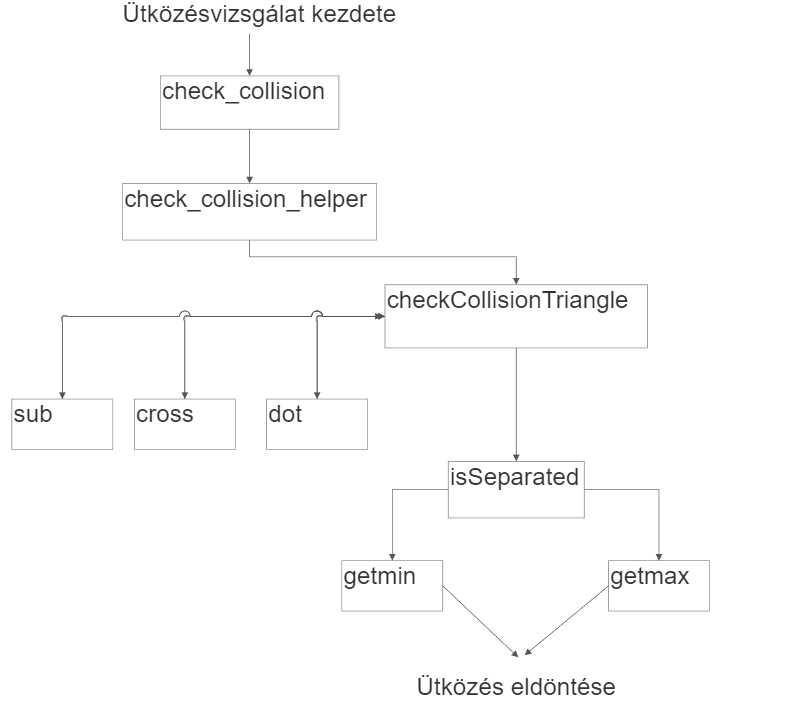
\includegraphics[width=15truecm, height=15truecm]{images/blokk_diagram.png}
	\caption{Függvénykönyvtár blokk diagramja}
	\label{fig:blokkdiagram}
\end{figure}


\newpage
\Section{Elemi szintű számítások}

Háromszöget metszéspontjának számításához több, a \textbf{C} nyelvbe alapértelmezetten be nem épített, szinte már elemi szintű függvényre van szükségünk. \\
Ilyen például a \textbf{minimum}, illetve \textbf{maximum} kiválasztása 3 \textbf{float}-ból a \textbf{math.h} függvénykönyvtár segítségével:

\begin{cpp}
float getmin(float a, float b, float c)
{
    return fminf(fminf(a, b), c);
}

float getmax(float a, float b, float c)
{
    return fmaxf(fmaxf(a, b), c);
}
\end{cpp}

Illetve az elemi szintű számítások, például 3 dimenziós vektorok \textbf{kivonása, szorzása Descartes szorzása}:

\begin{cpp}
vec3 sub(vec3 A, vec3 B)
{
    vec3 C;
    C.x = A.x - B.x;
    C.y = A.y - B.y;
    C.z = A.z - B.z;
    return C;
}
	
float dot(vec3 A, vec3 B)
{
    return A.x * B.x + A.y * B.y + A.z * B.z;
}
\end{cpp}
\newpage
\begin{cpp}
vec3 cross(vec3 A, vec3 B)
{
    vec3 C;
    C.x = A.y * B.z - A.z * B.y;
    C.y = -(A.x * B.z - A.z * B.x);
    C.z = A.x * B.y - A.y * B.x;
    return C;
}
\end{cpp}

Illetve a korábban említett eldöntés, hogy a két háromszög metszi-e egymást, vagy sem.

\begin{cpp}
bool isSeparated(float a1, float a2, float b0, float b1, float b2)
{
    float a0 = 0;
    if (fmaxf(getmin(a0, a1, a2), getmax(b0, b1, b2)) 
    == getmin(a0, a1, a2))
    {
        return true;
    }
    if (fmaxf(getmax(a0, a1, a2), getmin(b0, b1, b2)) 
    == getmin(b0, b1, b2))
    {
        return true;
    }
    return false;
}
\end{cpp}
\newpage
\Section{Metszéspont számítása}

Az előző szekcióban bemutatott számítások felhasználásával mostmár kiszámíthatjuk, hogy a háromszögek metszik-e egymást, vagy sem. Erre a \textbf{\texttt{check\_collision}} függvényt használjuk.

\begin{cpp}
bool check_collision(Model *model1, Model *model2, vec3 model1_position,
vec3 model2_position)
{
    int k = 0, l = 0;
    float limit, distance;
    limit = model1->farestpoint + model2->farestpoint + 0.5;
    distance = get_distance(model1_position, model2_position);
    if (fminf(distance, limit) == limit)
    {
        return false;
    }
    while (k < model1->i_f)
    {
        while (l < model2->i_f)
        {
            if (check_collision_helper(k, l, model1, model2, 
            model1_position, model2_position))
            {
                return true;
            }
            l++;
        }
        k++;
        l = 0;
    }
return false;
}
\end{cpp}

A függvénynek 4 bemenete van. Az első 2 bemenet adja meg, hogy melyik 2 modellt szeretnék leellenőrizni, hogy ütköznek-e. Az utolsó 2 bemenet adja meg a modellek jelenlegi pozícióját.
Elsőként leellenőrizzük a két modell közötti távolságot. Ha kiesnek egymás távolságából, akkor nem ellenőrizzük le a metszéseket, ezzel optimalizálva valamennyire a programot. 

Amennyiben közel vannak egymáshoz a modellek, akkor egy dupla ciklus segítségével végigmegyünk mindkét modell minden egyes háromszögén és leellenőrizzük, hogy ütköznek-e a \textbf{\texttt{check\_collision\_helper}} függvény segítségével. Ha ütköznek, akkor igaz értékkel visszatérünk, és nem ellenőrzünk tovább.
\newpage

Egyszerűbb olvashatóság kedvéért egy \textbf{\texttt{check\_collision\_helper}} segédfüggvényt használunk a metszéspontok számításához.

\begin{cpp}
bool check_collision_helper(int k, int l, Model *model1, 
Model *model2, vec3 model1_position, vec3 model2_position)
{
    vec3 A0, A1, A2, B0, B1, B2;
		
    A0.x = model1->v[model1->f[k].points[0].vertex_index].x 
    + model1_position.x;
    A0.y = model1->v[model1->f[k].points[0].vertex_index].y 
    + model1_position.y;
    A0.z = model1->v[model1->f[k].points[0].vertex_index].z 
    + model1_position.z;
    A1.x = model1->v[model1->f[k].points[1].vertex_index].x 
    + model1_position.x;
    A1.y = model1->v[model1->f[k].points[1].vertex_index].y 
    + model1_position.y;
    A1.z = model1->v[model1->f[k].points[1].vertex_index].z 
    + model1_position.z;
    A2.x = model1->v[model1->f[k].points[2].vertex_index].x 
    + model1_position.x;
    A2.y = model1->v[model1->f[k].points[2].vertex_index].y 
    + model1_position.y;
    A2.z = model1->v[model1->f[k].points[2].vertex_index].z 
    + model1_position.z;

    return checkCollisionTriangle(A0, A1, A2, B0, B1, B2);
}
\end{cpp}


6 bemenete van a függvénynek. Az első bemenet határozza meg, hogy az adott modell hanyadik háromszögét vizsgáljuk. A második bemenet határozza meg, hogy a másik modell hanyadik háromszögét vizsgáljuk. Utána következik a 2 modell, majd a modellek pozíciója.

Létrehozunk 6 darab 3 dimenziós vektort, amelyek tartalmazzák majd a háromszöget csúcspontjainak koordinátáit a térben. \\
Kiszámításának módja: \textit{model1->f[k].points[0].vertex\_index} \\
\textit{model1} az adott modell, amely egy pointerként rámutat az \textit{f} struktúrára, amely tartalmazza az adott háromszög adatait. Az \textit{f k}-adik indexű háromszögét vizsgáljuk mindig, azon belül a \textit{points} struktúrában tárolt adatokra van szükségünk. Ennek a változónak is a \textit{vertex\_index} elemére. Ezzel megkapjuk egy háromszög pontjának az indexét.

Ebből kinyerhetjük a háromszög csúcspontjainak pontos koordinátáit.

\textit{A0.x = model1->v[model1->f[k].points[0].vertex\_index].x 
	+ model1\_position.x}

Így beállíthatjuk az új háromszögünk első csúcspontjának X koordinátáját, amelyhez hozzá kell adnunk a modell jelenlegi pozícióját. Ezt megismételjük mindig csúcspontra, illetve a másik modellre is, mielőtt meghívjuk a \textbf{checkCollisionTriangle} függvényt.

\newpage

A \textbf{checkCollisionTriangle} függvény megkapja az előző függvény által kiszámolt 6 csúcspontot. Ezen csúcspontok segítségével számolja ki a fentebb említett számolási módszer segítségével az éleket, a normál vektorokat és a távolságot, majd leellenőrzi, hogy a háromszöget metszik-e egymást, vagy sem.

\begin{cpp}
bool checkCollisionTriangle(vec3 A0, vec3 A1, vec3 A2, vec3 B0,
vec3 B1, vec3 B2)
{
    vec3 C0 = sub(A1, A0);
    vec3 C1 = sub(A2, A0);
    vec3 C2 = sub(C1, C0);
    vec3 D = cross(C0, C1);
    vec3 E0 = sub(B1, B0);
    vec3 E1 = sub(B2, B0);
    vec3 E2 = sub(E1, E0);
    vec3 F = cross(E0, E1);
    vec3 G = sub(B0, A0);
}
\end{cpp}

A metszések kiszámítása kódban terjedelmes, ezért csak 1 példa lesz bemutatva.

\begin{cpp}
float h1, i0, i1, i2;
	
// Separate: D
i0 = dot(D, G);
i1 = i0 + dot(D, E0);
i2 = i0 + dot(D, E1);
if (isSeparated(0, 0, i0, i1, i2))
{
    return false;
}
\end{cpp}

Itt a \textit{D} normálvektor alapján próbáljuk eldönteni, hogy különállnak-e a háromszögek, vagy sem. A táblázat alapján kiszámítjuk a \textit{$H_1, H_2, I_0, I_1, I_2$} változókat, majd az alapján meghívjuk az \textit{isSeparated} függvényt, amely eldönti, hogy a háromszögek különállnak-e, vagy sem. (Az \textit{isSeparated} függvény megtalálható az "Elemi szintű számítások" szekcióban)
\newpage

\Section{Modell formázása}

Az eddig bemutatott kódok alapján a program így csak az alapértelmezett modelleket képes kezelni, ami nem kedvező számunkra. Ezért új függvények lettek létrehozva a modellek méretezéséhez, forgatásához, tükrözéséhez. Ha azt szeretnénk, hogy a modell "hitboxa" mozogjon a modellel együtt, akkor ezeket a függvényeket kell használnunk az \textbf{OpenGL}-ben alapértelmezett függvények helyett. Ezek a függvények magát a modellt módosítják, nem pedig a megjelenítését.

\subsection{Modell méretezése}

\begin{cpp}
void scale_model(Model *model, float scalex, float scaley, 
float scalez)
{
    int k = 0;
    while (k < model->i_f)
    {
        for (int i = 0; i < 3; i++)
        {
            model->v[k].x *= scalex;
            model->v[k].y *= scaley;
            model->v[k].z *= scalez;
        }
			
        k++;
    }
}
\end{cpp}

A \textbf{scale\_model} függvény 4 bemenettel rendelkezik, az első a modell maga, a maradék 3 pedig a méretezéshez szükséges float változók. A függvény végigmegy minden egyes háromszögén a modellnek, és a háromszög csúcspontjainak a koordinátáit megszorozza a megadott új méretekkel. Modellek méretezéséről példát a \ref{fig:meret_1}, illetve \ref{fig:meret_2} ábrákon láthatunk.
\newpage

\begin{figure}[h]
	\centering
	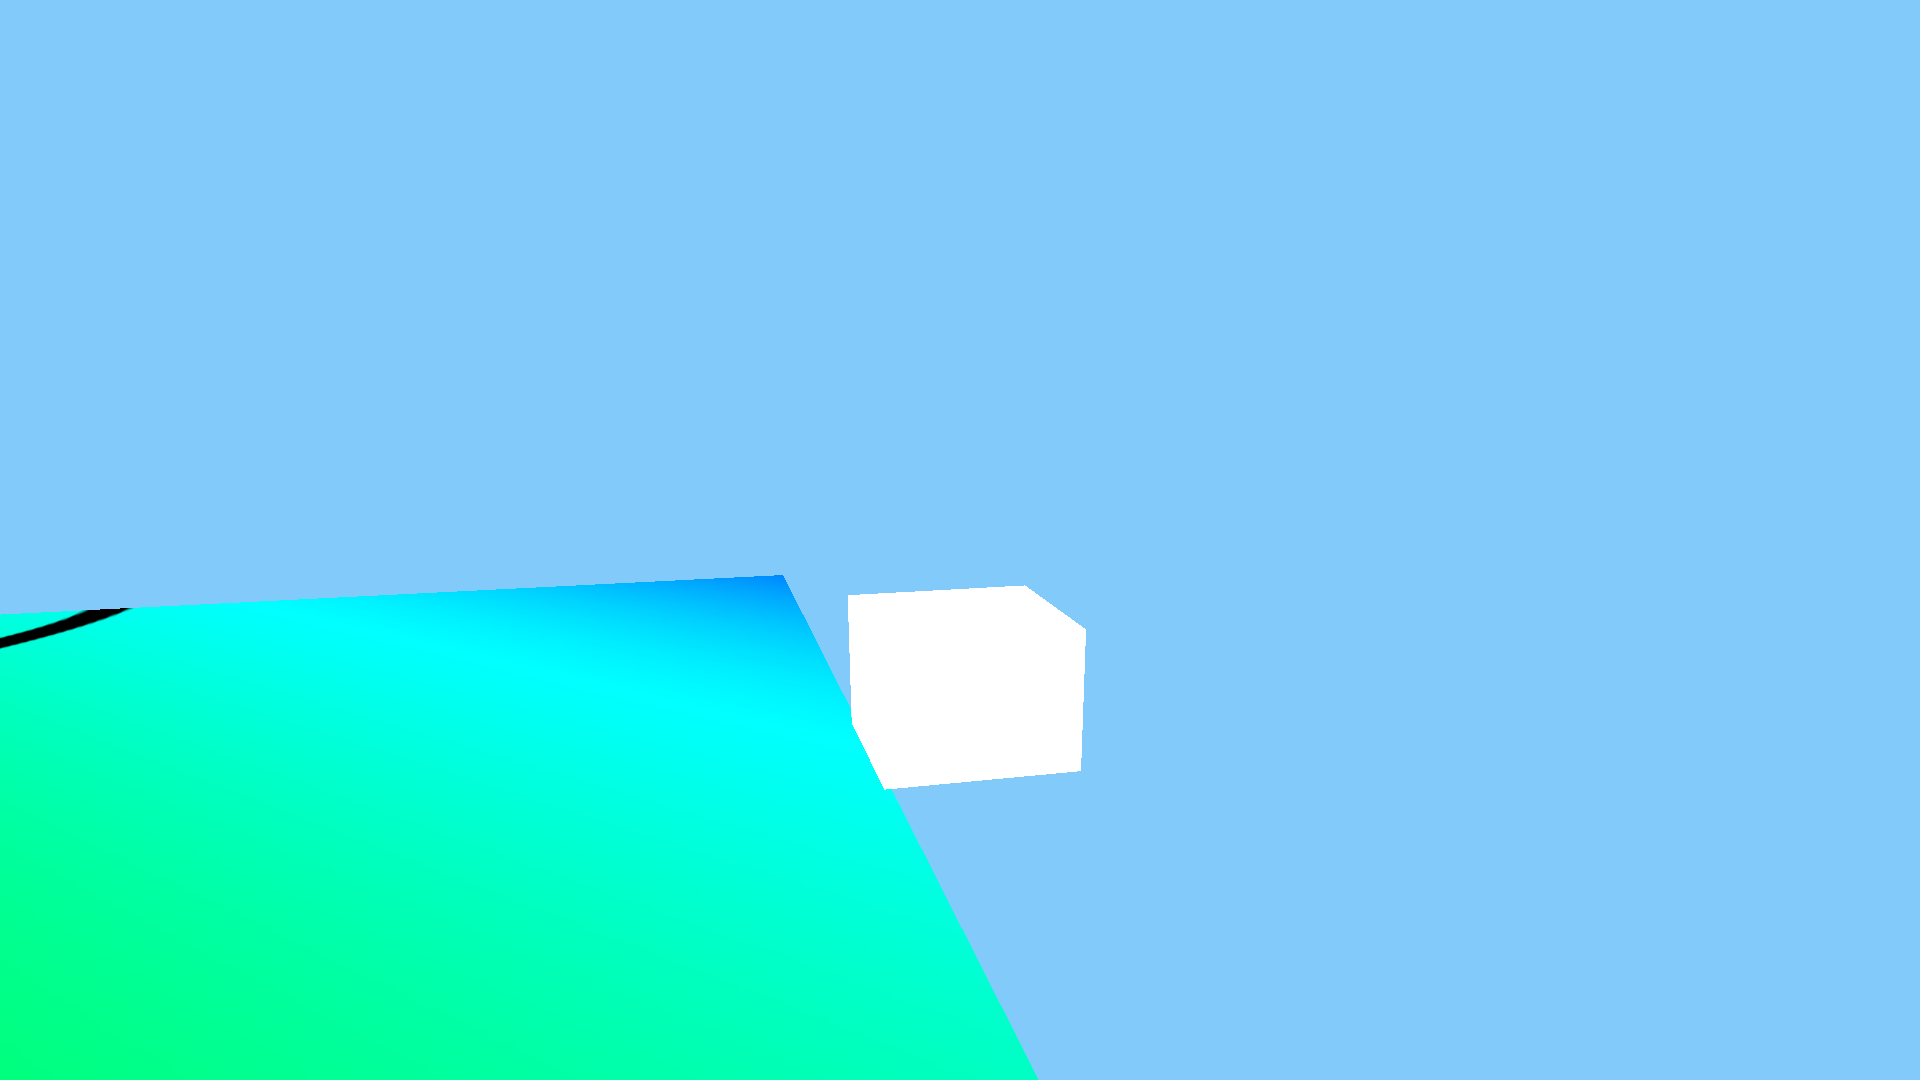
\includegraphics[width=13truecm, height=7truecm]{images/modell_4.3.1.1.png}
	\caption{Alapértelmezett playermodell méret}
	\label{fig:meret_1}
\end{figure}

	$$\big\Downarrow$$
	
	
\begin{figure}[h]
		\centering
		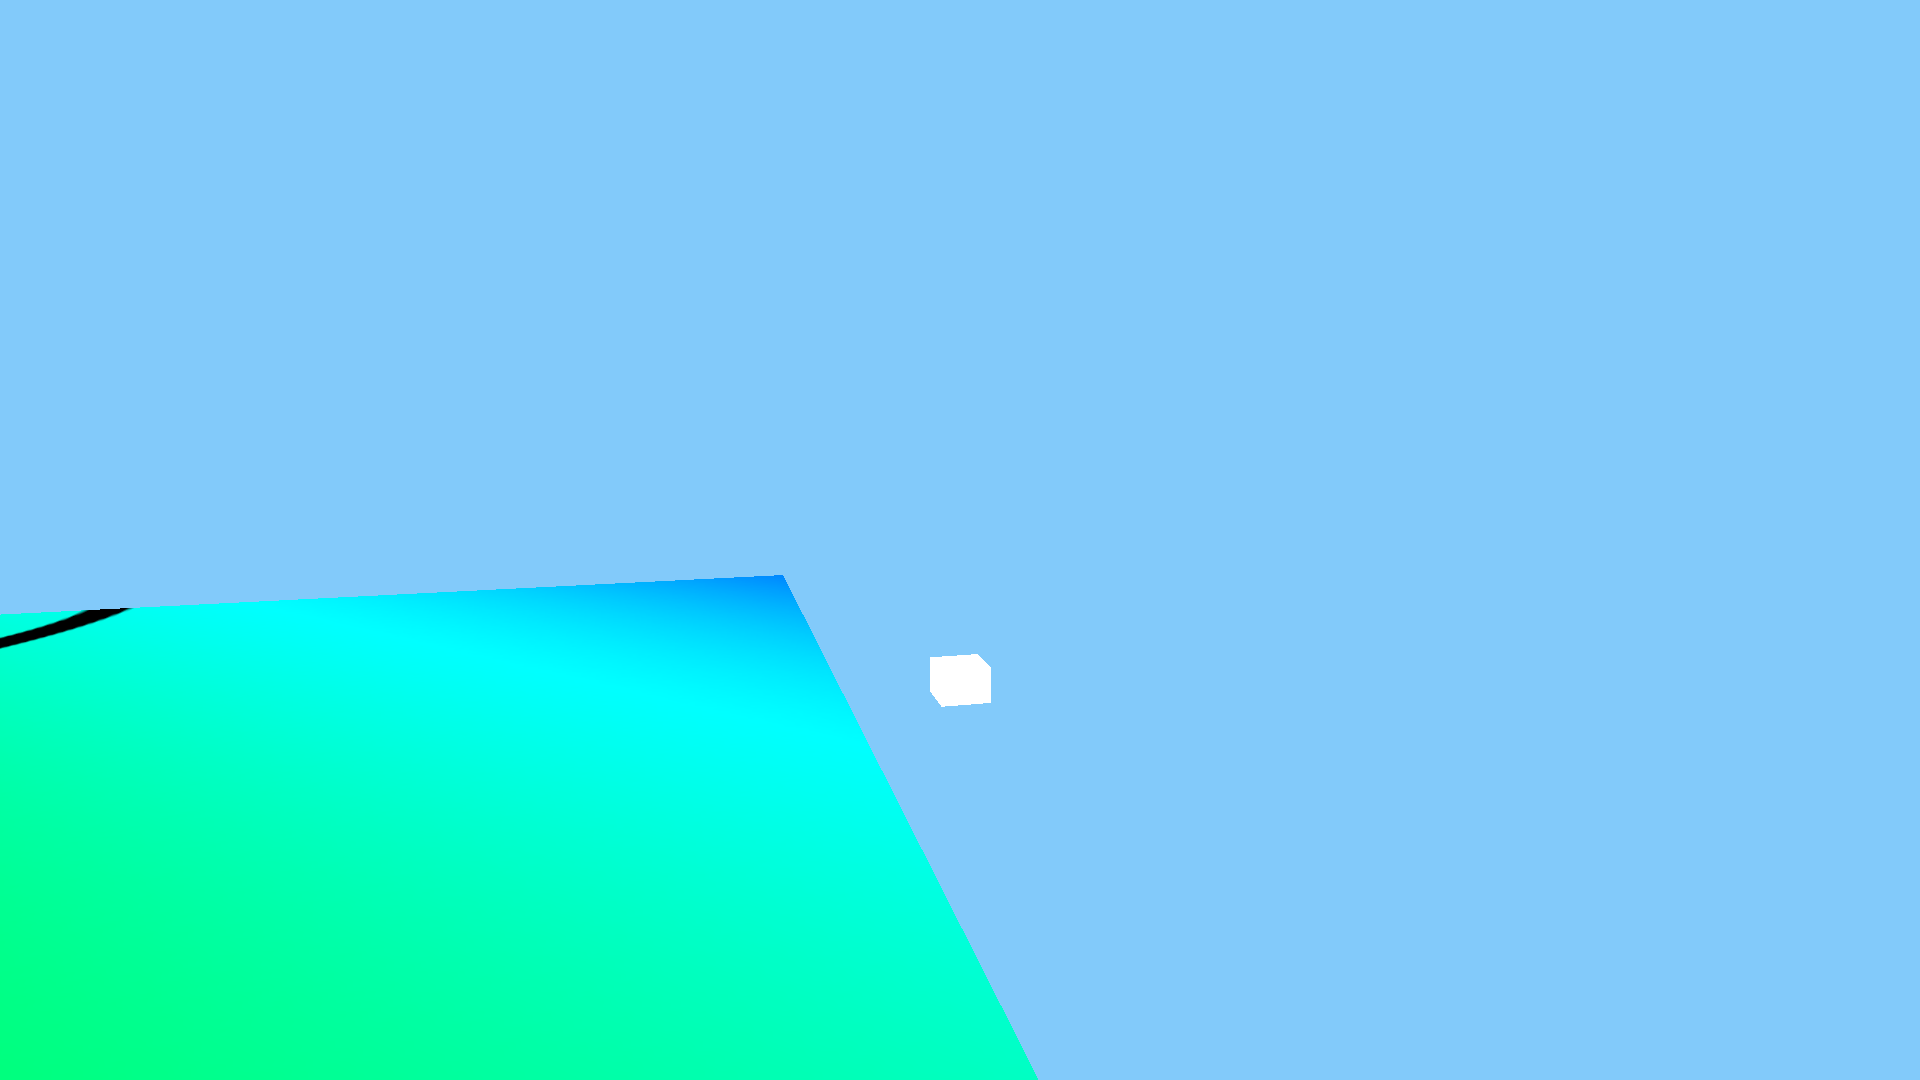
\includegraphics[width=13truecm, height=7truecm]{images/modell_4.3.1.3.png}
		\caption{Playermodell méretének csökkentése}
		\label{fig:meret_2}
\end{figure}

	



\newpage
\subsection{Modell forgatása}

\begin{cpp}
void rotate_model(Model *model, float anglex, float angley, float anglez)
{
    int k = 0;
    float cord1, cord2, angle;
    while (k < model->i_f)
    {
        cord1 = model->v[k].x;
        cord2 = model->v[k].y;
        angle = anglex * (float)(M_PI / 180);
        model->v[k].x = cord1 * cosf(angle) - cord2 * sinf(angle);
        model->v[k].y = cord1 * sinf(angle) + cord2 * cosf(angle);
			
        cord1 = model->v[k].x;
        cord2 = model->v[k].z;
        angle = angley * (float)(M_PI / 180);
        model->v[k].x = cord1 * cosf(angle) - cord2 * sinf(angle);
        model->v[k].z = cord1 * sinf(angle) + cord2 * cosf(angle);
			
        cord1 = model->v[k].y;
        cord2 = model->v[k].z;
        angle = anglez * (float)(M_PI / 180);
        model->v[k].y = cord1 * cosf(angle) - cord2 * sinf(angle);
        model->v[k].z = cord1 * sinf(angle) + cord2 * cosf(angle);
        k++;
    }
}
\end{cpp}

A modell forgatása az egyik legnehezebb feladat az összes közül. Itt nem elég szimplán szoroznunk, hanem a forgatás miatt \textbf{cos}inus, illetve \textbf{sin}us számításokat is végeznünk kell. A függvény végigmegy minden egyes háromszögén a modellnek, majd a csúcspontok koordinátáit módosítja \textbf{sin}us és \textbf{cos}inus számítással az adott forgatási szögek alapján. Modellek forgatásáról példát a \ref{fig:forgatas_1}, illetve \ref{fig:forgatas_2} ábrákon láthatunk.

\newpage

\begin{figure}[h]
	\centering
	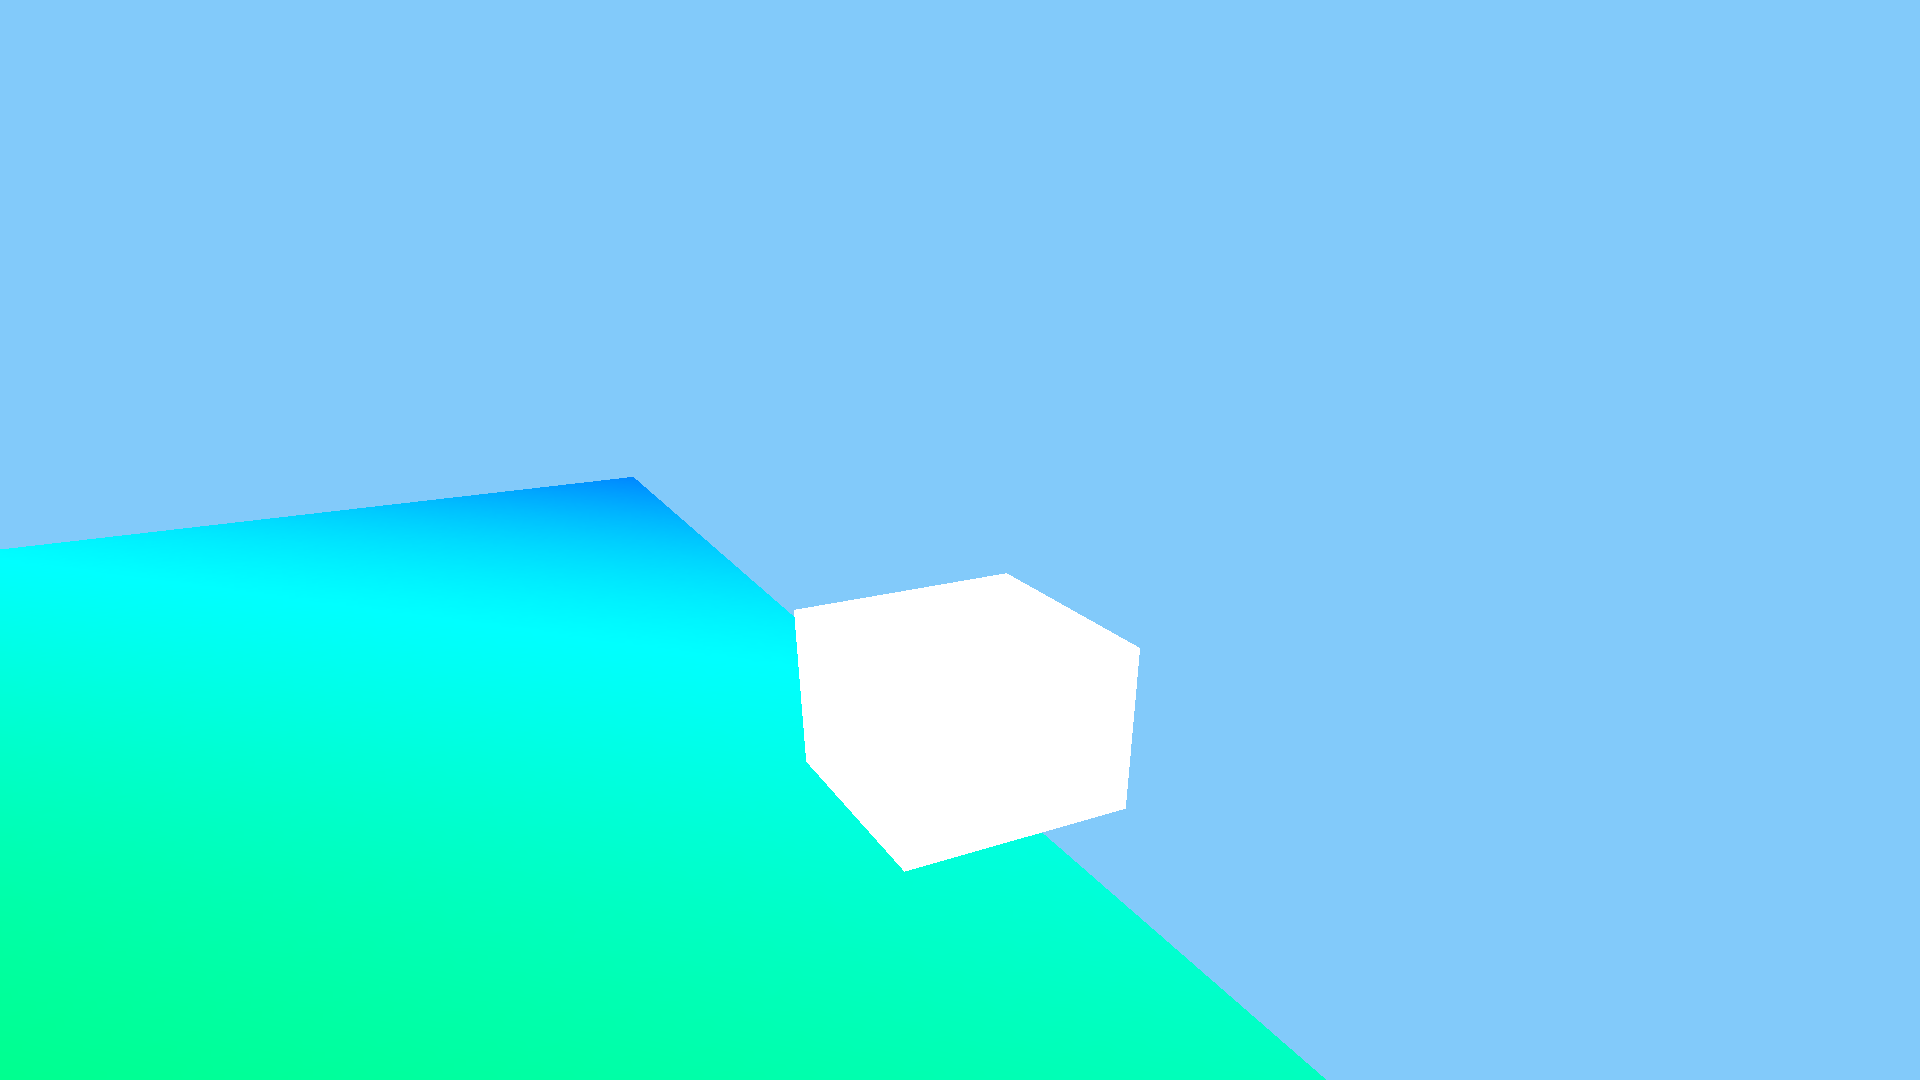
\includegraphics[width=13truecm, height=7truecm]{images/modell_4.3.2.1.png}
	\caption{Alapértelmezett playermodell forgatás}
	\label{fig:forgatas_1}
\end{figure}
$$\big\Downarrow$$
\begin{figure}[h]
	\centering
	
\includegraphics[width=13truecm, height=7truecm]{images/modell_4.3.2.3.png}
	\caption{Playermodell forgatása a tengelyeken}
	\label{fig:forgatas_2}
\end{figure}






\newpage